\documentclass[twoside,11pt,a4paper,english]{article}

% packages %%%%%%%%%%%%%%%%%%%%%%%%%%%%%%%%%%%%%%%%%%%%%%%%%%%%%%%%%%%%%%%%%%%%
\usepackage{graphicx,curves,float,rotating}

\usepackage{amsmath, amssymb, latexsym}  % math stuff
\usepackage{amsopn}                             % um mathe operatoren zu deklarieren
\usepackage[english]{babel}                     % otherwise use british or american
\usepackage{theorem}                            % instead of \usepackage{amsthm}
\usepackage{dcolumn}
\usepackage{hyperref}
\usepackage[]{algorithm2e}
\usepackage{float}


% @ environment %%%%%%%%%%%%%%%%%%%%%%%%%%%%%%%%%%%%%%%%%%%%%%%%%%%%%%%%%%%%%%%%
\usepackage{xspace}                             % context sensitive space after macros
\makeatletter 
\DeclareRobustCommand\onedot{\futurelet\@let@token\@onedot}
\def\@onedot{\ifx\@let@token.\else.\null\fi\xspace}
\def\eg{{e.g}\onedot} \def\Eg{{E.g}\onedot}
\def\ie{{i.e}\onedot} \def\Ie{{I.e}\onedot}
\def\cf{{c.f}\onedot} \def\Cf{{C.f}\onedot}
\def\etc{{etc}\onedot} \def\vs{{vs}\onedot} 
\def\wrt{w.r.t\onedot} \def\dof{d.o.f\onedot}
\def\etal{{et al}\onedot}
\def\zB{z.B\onedot} \def\ZB{Z.B\onedot}
\def\dh{d.h\onedot} \def\Dh{D.h\onedot}
% %%%%%%%%%%%%%%%%%%%%%%%%%%%%%%%%%%%%%%%%%%%%%%%%%%%%%%%%%%%%%%%%%%%%%%%%%%%%%%%


%	Macros fuer neue Umgebungen
  

%%%%%%%%%%%%%%%%%%%%%%%%%%%%%%%%%%%%%%%%%%%%%%%%%%%%%%%%%%%%%%%%%%%%%%%%%%%%%%
\newcommand*{\Frac}[2]{\frac{\displaystyle #1}{\displaystyle #2}}
\newlength{\textwd}
\newlength{\oddsidemargintmp}
\newlength{\evensidemargintmp}
\newcommand*{\hspaceof}[2]{\settowidth{\textwd}{#1}\mbox{\hspace{#2\textwd}}}
\newlength{\textht}
\newcommand*{\vspaceof}[3]{\settoheight{\textht}{#1}\mbox{\raisebox{#2\textht}{#3}}}
\newcommand*{\PreserveBackslash}[1]{\let\temp=\\#1\let\\=\temp}
\newcommand{\reals}{\mathbb{R}}

\newenvironment{deflist}[1][\quad]%
{  \begin{list}{}{%
      \renewcommand{\makelabel}[1]{\textbf{##1}\hfil}%
      \settowidth{\labelwidth}{\textbf{#1}}%
      \setlength{\leftmargin}{\labelwidth}
      \addtolength{\leftmargin}{\labelsep}}}
{  \end{list}}


\newenvironment{Quote}% Definition of Quote
{  \begin{list}{}{%
      \setlength{\rightmargin}{0pt}}
      \item[]\ignorespaces}
{\unskip\end{list}}


\theoremstyle{break}
\theorembodyfont{\itshape}	
\theoremheaderfont{\scshape}

\newtheorem{Cor}{Corollary}
\newtheorem{Def}{Definition}
%\newtheorem{Def}[Cor]{Definition}



\newcolumntype{.}{D{.}{.}{-1}}


\pagestyle{headings}
\textwidth 15cm
\textheight 23cm
\oddsidemargin 1cm
\evensidemargin 0cm
%\parindent 0mm



%%%%%%%%%%%%%%%%%%%%%%%%%%%%%%%%%%%%%%%%%%%%%%%%%%%%%%%%%%%%%%%%%%%%%%%%%%%%%%%
%
%
%       Jetzt geht's los
%
%
%%%%%%%%%%%%%%%%%%%%%%%%%%%%%%%%%%%%%%%%%%%%%%%%%%%%%%%%%%%%%%%%%%%%%%%%%%%%%%%
\begin{document}


%%%%%%%%%%%%%%%%%%%%%%%%%%%%%%%%%%%%%%%%%%%%%%%%%%%%%%%%%%%%%%%%%%%%%%%%%%%%%%%
%
%
%               Title
%
%
%%%%%%%%%%%%%%%%%%%%%%%%%%%%%%%%%%%%%%%%%%%%%%%%%%%%%%%%%%%%%%%%%%%%%%%%%%%%%%%
\pagestyle{empty}

\begin{center}

    Rheinisch-Westf\"alische Technische Hochschule Aachen \\
    Lehrstuhl f\"ur Informatik 6 \\
    Prof. Dr.-Ing. Hermann Ney\\[6ex]
    Seminar Titel im SS 2018\\[12ex]                          % auch Seminar Titel und Datum �ndern!!!
   
    \LARGE
    \textbf{Deep Clustering for ANN Supported Source Separation } \\[6ex]
    \textit{Patrick von Platen} \\[6ex]
    \Large
    Matrikelnummer 331 430 \\[6ex]
    19.06.2018	

    \vfill
    \Large Betreuer: Tobias Menne 
	    
\end{center}

\newpage
\ 
\newpage

%%%%%%%%%%%%%%%%%%%%%%%%%%%%%%%%%%%%%%%%%%%%%%%%%%%%%%%%%%%%%%%%%%%%%%%%%%%%%%%
%
%
%               Inhaltsverzeichnis / Tabellenverzeichnis / Abbildungsverz.
%
%
%
%%%%%%%%%%%%%%%%%%%%%%%%%%%%%%%%%%%%%%%%%%%%%%%%%%%%%%%%%%%%%%%%%%%%%%%%%%%%%%%
\pagestyle{headings}
\tableofcontents
\listoftables
\listoffigures
\newpage
\pagestyle{empty}
\ 
\newpage
\pagestyle{headings}

\section{Introduction} % (fold)
\label{sec:introduction}

When perceiving sound created by multiple acoustic sources, the human auditory system
is extremely good at focussing on parts of the sound coming from only one acoustic
source.

Imagine yourself at a cocktail party. The sound that you perceive is made up of all kinds of acoustic sources: The voice of the person you are listening to, the sound of music,
the background chatter of other people talking, the sound of clinking glasses, etc. Still you can clearly understand the speaker in your group, even though its acoustic signal overlaps at every moment with the acoustic signal of other people speaking and background noise. 

The difficulty of understanding speech in a multiple speaker environment is often called "The cocktail party problem" \cite{CocktailPartyProblem:2000}, first mentioned by Colin Cherry in 1953. 
It was also Colin Cherry, who first brought up the idea of automatic speech separation in his famous paper on ``experiments of the recognition of speech'' \cite{Cherry:1953}.
The first method to yield some promising results was introduced by A.S. Bregman in 1990 using \emph{Auditory scene analysis} \cite{bregman1994auditory}.
Since then, multiple methods have been explored. One of them is \emph{Spectral Clustering}
, a method based on partitioning data points into clusters according to the eigenstructure
of a similarity matrix. 

With the receent rise of deep learning in a variety of applications, the first method
to be applied to source separation was presented by Chao Weng and co. in 2015 \cite{SpeechSepDeepLearning:2015}. 
Quickly, different deep learning methods based on a technique called \emph{Deep Clustering} emerged, forming the state-of-art in the source separation problem. 
This report, will focus on the deep clustering method as it was introduced by John R. Hershey and co. in 2015 \cite{BasicDeepClustering:2016} and will study \emph{TasNet}, a deep clustering system performing audio separation in the time domain yielding state-of-the art results \cite{TasNet}.

The applications of automated source separation are wide-ranging. To name a few: 
\begin{itemize}
	\item \textit{Automatic meeting transcription}: In business meetings, multiple speakers are alteranating in a short time or even speaking at the same time. Making it possible to automatically separate speakers from each other and transcribe would be of great use for companies. 
	\item \textit{Virtual assistant}: Virtual assistants, like Alexa, Siri and Google Home are playing a critical part in smart home systems. Filtering out noise and separating the owner's voice from other voices are challenges that can be taken on by automated source separation techniques. 
	\item \textit{Automatic subtitling of music/video}: According to the World Health Organization (WHO) over 5\% of the world population suffers from disabling hearing loss \cite{HearingLoss}. Subtitling of music and video content, which are often made up of sound coming from multiple acoustic sources, is therefore essential for them.	
\end{itemize}

To begin with, the source separation problem is mathematically defined and basic mathematical operations and basic deep learning methods used in deep clustering are explained \ref{sec:basics}.
In the following conventional methods and first attempts of using deep learning techniques for automated source separation are presented \ref{sec:conventional_methods}.
		The essence of this paper being deep clustering and \emph{TasNet} will be presented in-detail in section \ref{sec:deep_clustering_methods}. 
Finally, a conclusion is drawn \ref{sec:conclusion}.
% section introduction (end)

\section{Basics} % (fold)
\label{sec:basics}

This section firstly defines the source separation problem and then gives an 
overview of the basic operations and methods used in the later presented systems.

\subsection{Definition source separation problem} % (fold)
\label{sec:source_separation_problem}

A generel definition of the source separation problem was given by Jean-Francois Cardoso, 
defininig the problem as ``recovering unobserved signals or sources from several
observed mixtures'' \cite{Cardoso03blindsignal}. He also added two important restrictions that we will apply to our definition as well: 
\begin{enumerate}
 \item The source signals are not observed
 \item No information is available about the mixture
\end{enumerate}

The condition of not knowing how many sources the mixture is composed of became known as \emph{blind} source separation \cite{Cardoso03blindsignal}. 
In this paper, we add another restriction: The signal is observed over a single channel (single microphone).
To sum it up, the \emph{source separation problem} is defined in this paper as ``recovering the original signals of an unknown amount of sources from a single-channel mixture of the source signals''.

Putting the above definiton in a mathematical form:
\begin{itemize}
	\item the unknown number of acoustic sources: $N$.
	\item the original sound of the i-th source at time t: $x_i(t)$.
	\item the single received sound signal at time t: $x(t) = \sum_{i=1}^{N} x_i(t)$.
\end{itemize}

The goal of source separation is to recover $x_1(t),...,x_N(t)$ from $x(t)$.
An algorithm performing this task is presented below.

\begin{algorithm}[ht]
	\RestyleAlgo{boxruled}
	\LinesNumbered
	\textbf{Input: }$x(t)$ \\
	\textbf{Output: }$(N, \{x_1(t), ..., x_N(t)\})$
\end{algorithm}

% section source_separation_problem (end)

\subsection{Mathematical operations} % (fold)
\label{sub:mathematical_oprations}

This section aims to shine light on essentiel 
mathematical operations used in the systems that will 
be explained in sections \ref{sec:conventional_methods}, \ref{sec:deep_clustering_methods}. 

\subsubsection{Short term fourier transform} % (fold)
\label{ssub:short_term_fourier_transform}

In order to understand the short term fourier transform, one firstly has to get an understanding of the fourier transform itself. Having a continous signal $s(t)$, the fourier transform is defined as

\[
	S(f) = \int_{\mathbb{R}} s(t) e^{-2j{\pi}ft} dt
\]

The fourier transform $S(f)$ gives the magnitude of every frequency in the signal. A signal can be decomposed as the sum of signals consisting only of one frequency (so called sinusoids).
 Thus, one can say that the higher the magnitude of a frequency of the fourier transform, the higher is the percentage of the signal being composed of the sinusoid of
 this frequency. An important aspect to notice is that the fourier transform
 integrates over the whole time domain of the signal in order to get the exact magnitude
 of every freuency present in the signal. Thus integrating only over a part of the time domain leads
 to approximated values of the frequencies magnitudes. On the other hand, a shorter time
 intervall to integrate over leads to a better time localization of the frequency. This famous
 trade-off is well-known as the uncertainty principle in signal analysis \cite{DBLP:journals/corr/Nam13}.

The short term fourier transform divides the signal into local sections using a window function $w(\tau) = 0 : \tau \not \in \left[-a, a \right]$ over which the fourier transform is applied.  
\[
	S(f,t) = \int_{\mathbb{R}} s(\tau)w(\tau-t) e^{-2j{\pi}f\tau} d\tau 
\]

Appling the short term fourier transform converts a signal $X(t)$ to multiple $(F,T)$ bins that can be plotted in a \emph{spectrogram} as can be seen in Figure \ref{fig:spectrogram}. It therefore is used to describe the change in frequency over time. Using an appropiate window funciton leads to a good trade-off between time localization and frequency approximation.

\begin{figure}[H]
	\centering
	\includegraphics[width=0.8\linewidth]{images/spectogram.png}
	\caption{Spectrogram of a speech signal}
	\label{fig:spectrogram}
\end{figure}

% subsubsection short_term_fourier_transform (end)

\subsubsection{Embedding space} % (fold)
\label{ssub:embedding_space}

An embedding is a structure-preserving, injective mapping $f: X \to Y$. Therefore, every
object of domain $X$ is mapped to a distinct object in domain $Y$. In this report, we are
interested in embeddings that map to normed spaces meaning that it is possible to measure
the similarity of two objects $x_1,x_2 \in X$ by measuring its distance $d(y_1, y_2) \in \mathbb{R}: y_1, y_2 \in Y$.
It is essentially used to convert data to a feature representation where certain properties can be preserved by distance, so that the data is easily comparable by computers.

One famous example are word embedding models, such as \emph{word2vec} that maps words
to a vector representation. Assuming that words have multiple degrees of similarity, word
embeddings are used to quantisize the similarity of words on multiple axis \cite{DBLP:journals/corr/abs-1301-3781}.
Later, we will see that the function mapping objects from one domain to an embedding
space can be trained on artificial neural networks and are very powerful tools for the source separation problem \ref{sub:frequency_domain_audio_separation}.

\subsection{Deep neural network basics} % (fold)
\label{sub:deep_neural_network_basics}

This section aims to clarify basic deep learning methods and architectures used in the sections \ref{sec:conventional_methods}, \ref{sec:deep_clustering_methods}.

\subsubsection{Convolutional neural network}%
\label{ssub:convolutional_neural_network}

Convolutional neural networks are neural networks that are specialized for processing 
data that has grid-like topology, for example time series data for a 1D convolution \cite{Goodfellow-et-al-2016}. 
The idea is based on the convolution operation $*$ being:

\[
	s(t) * g(t) = \int_{\reals} s(\tau) g(t - \tau) d\tau
\]

which corresponds to 

\[
	s(n) * g(n) = \sum_{i = -\infty}^{\infty} s(i) g(n - i)
\]

in the discrete case. The fourier transform of a signal to its spectrum can essentially 
be seen as a convolution operation \cite{664179}.

This principle can now be applied to artificial neural networks. Let $x$ be the output 
layer and $w$ the weights of a convolutional layer. Such a layer is defined by its 
filter size $k$ and other parameters, such as stride, padding, etc. For more information 
please refer to \cite{Goodfellow-et-al-2016}. The weight array is also called 
``Kernel'' \cite{DBLP:journals/corr/SunOO15} and normally a convolutional layer is 
decomposed of multiple kernels, such that there are multiple parallel outputs. 
The convolution operation in neural networks is defined as follows:

\[
	y_{i,j} = w_i * x = f(\sum_{n = j}^{j+k}(w_{i,n - j} x_n) + b_i)
\]

$y_{i,j}$ presents the j-th neuron of the output layer of the i-th kernel.
Similarly $w_{i,l}$ presents the l-th weight of the i-th kernel. $x_n$ is the output of the n-th neuron of the previous layer and $b_i$ is the bias corresponding to the i-th kernel.
Finally $f()$ is the activation function applied to each convolution operation. 

Convolutional neural networks can very well be applied to act as filterbanks for the signal as was shown in \cite{Golik2015ConvolutionalNN} and as we will later see in section
\ref{sub:frequency_domain_audio_separation}.

\subsubsection{Recurrent neural network} % (fold)
\label{ssub:recurrent_neural_network}

Recurrent neural networks are neural networks that are ``specialized in processing a sequence
of values $x_1,...,x_t$'' \cite{Goodfellow-et-al-2016}. For that reason, they are very well applicable when dealing
with acoustic signals having high autocorrelation (high correlation between $s(t)$ and
$s(t - k), s(t + k)$  for $k > 0$).
Recurrent neural networks are extremely effective when dealing with sequential data.
First, they process data of different time instances in one computation
step, thus taking full advantage of autocorrelation. Second, they can handle data
sequences of variable length in contrast to feed forward neural networks where the input length is determined by the size of the input layer. 
This is achieved by loops between
recurrent units inside the neural network \cite{Goodfellow-et-al-2016}.
Unfolding a recurrent unit $z$ of a recurrent neural network at different time instances
leads to so-called hidden copies of the network being connected to each other: $z^0, z^1, ..., z^{t-1}, z^{t}$
As a result, such a recurrent unit $z^t$ at time t takes both the output of the node leading
to it ($x^t$) and the output of the same recurrent unit of one time instance earlier $(z^{t-1})$ as input resulting in:

\[
	z^t =f(V x^t + Wz^{t-1} + b)
\]
with $f()$ being the activation function, V the weights between recurrent unit z and input
x, W the weights between two hidden recurrent units $z^{t-1}$ and $z^t$ and b the constant bias term.
This basic setup is known to have the vanishing/exploding gradient problem due to an
exponential decrease/increase in value of long-term components ($\frac{\partial z^t}{\partial z^{t-k}} \to \text{ \textit{const.}} \times W^{k} \to 0 \text{ or } \infty$
)\cite{Pascanu:2013:DTR:3042817.3043083}. To overcome this problem, Hochreiter and co. introduced a ``better'' recurrent unit,
called long shot term memory.

% subsubsection recurrent_neural_network (end)

\subsubsection{Long short term memory} % (fold)
\label{ssub:long_short_term_memory}

To overcome the exploding/vanishing gradients problem, the long short term memory unit
introduces an internal state which can be seen as the unit's ``memory'' \cite{Hochreiter:1997:LSM:1246443.1246450}. At every time
instance t, the unit updates its memory $c^t$ using the memory $c^{t-1}$ and the unit's output
$h^{t-1}$, as well as the new input $x^t$. $c^t$ in combination with $h^{t-1}$ and $x^t$ is then used to
produce the new output. The structure of the long short term memory unit is shown in
Figure \ref{fig:lstm}. It is important to notice that the long short term memory uses $x^t$ and $h^{t-1}$ to
compute four different gates: f,i,g,o which are used to control the 
flow of information in
the unit. Also, we can see that when doing backpropagation, the gradient easily ``flows'' to
earlier hidden units without the weight matrix being applied to it (shown by the red arrow) in \ref{fig:lstm}.
This ``highway'' for the gradient strongly reduces the vanishing/exploding gradient
effect and allows the unit to take into account long term dependencies of the input data.

\begin{figure}[h!]
  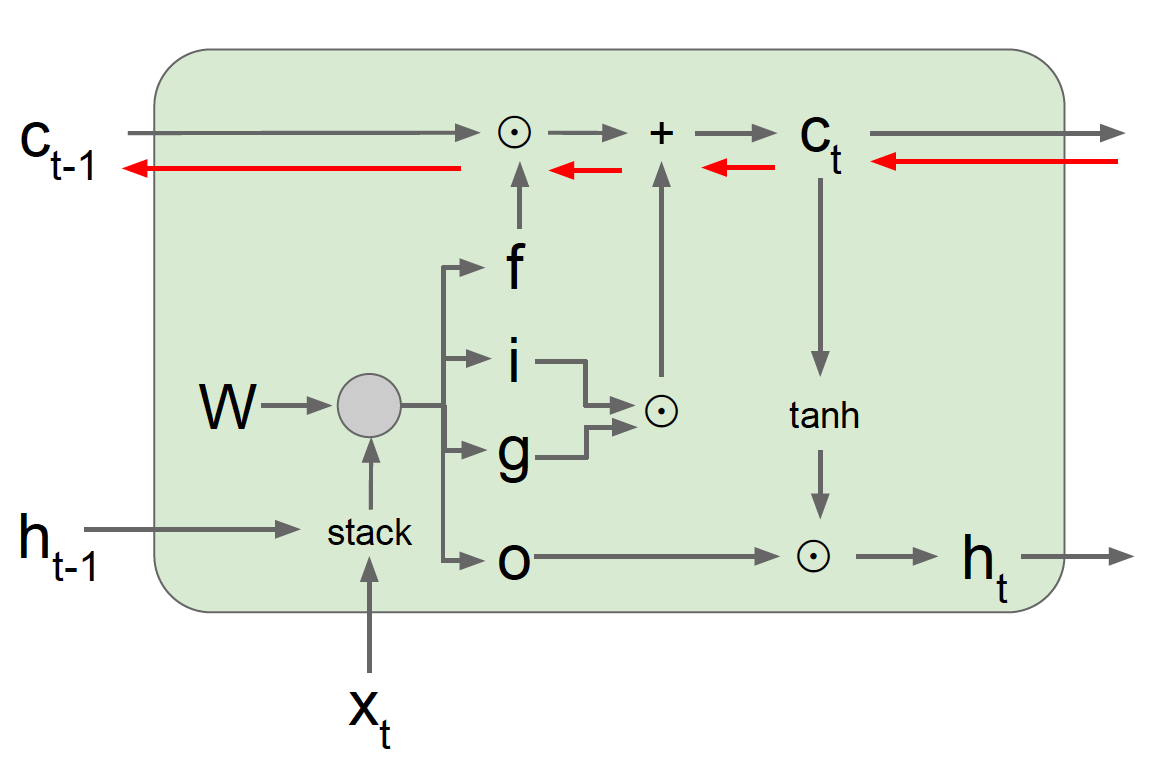
\includegraphics[scale=0.4]{images/lstm_structure.png}
  \centering
  \caption{Long short term memory}
  \label{fig:lstm}
\end{figure}

To furter improve this ability, bi-directional long short term memory units were proposed
to exploit correlations between data in both time directions and are used in many
state-of-the-art systems nowadays. Going more into detail is out of scope for this report,
but more informationcan be found in \cite{Hochreiter:1997:LSM:1246443.1246450}.

% subsubsection long_short_term_memory (end)

\subsubsection{Autoencoder}

An autoencoder is a neural network that is ``trained to attempt to copy its input to its
output'' \cite{Hochreiter:1997:LSM:1246443.1246450}. It always consists of two parts, the encoder and the decoder. In its simplest
form, the encoder maps the input x to one hidden layer $f(x) = z$ and the decoder tries to
reconstruct the original data $g(z) = x'$ from this layer.
Even though autoencoders are trained with loss functions trying to minimize the difference
between $x$ and $x'$, perfect recontruction of the data input is not the goal. Instead,
autoencoders should be trained in a way preventing them to just copy the input to the
output, but to extract useful information about data distribution instead \cite{Goodfellow-et-al-2016}. Thereby, the
hidden layer should represent the most useful information. 

Two approaches are considered
in this report.
First, a undercomplete autoencoder is defined by the hidden layer having much lower
dimension than the data, thus forcing the network to ``store all data in a compressed form''.
A backdraw of this approach is that the hidden layer might be two small to learn enough
useful information. Second, a sparse autoencoder forces the hidden layer to be sparse, by
introducing a sparsity penalty on the hidden layer $P(h)$, which will then be added to the
loss function $\mathbb{L}(x,x')+P(h)$. Especially in the field of machine translation, autoencoders
in combination with recurrent neural networks produce state-of-the-art results \cite{DBLP:journals/corr/abs-1801-05119}. 
For more detailed information, please refer to \cite{Goodfellow-et-al-2016}.

% subsection deep_neural_network_basics (end)
% section basics (end)

\section{Conventional methods} % (fold)
\label{sec:conventional_methods}

The first theoretical framework for automated source separation was introduced by A.S. Bregman in 1990 \cite{bregman1994auditory}. Systems using this approach are called \emph{computational auditory scene analysis} and produced first results which are 
acceptable \cite{4429320}. Section \ref{sub:computational_auditory_scene_analysis} will 
cover this method. 

\emph{Spectral Clustering}, a method well-know for data clustering, was then applied 
to the source separation problem and showed good results
(see \ref{sub:spectral_clustering}). 
It was the first method used for source separation to train some of its parameters on actual data \cite{Bach:2006}. 

\subsection{Computational auditory scene analysis}%
\label{sub:computational_auditory_scene_analysis}

Computational auditory scene analysis for source separation is an automation of the auditory scene analysis 
which is inspired by the principles of processing sound in human auditory system \cite{4429320}. 
In computational auditory scene anlysis the algorithm consists of two parts: \emph{segmentation} and \emph{grouping}. A more detailed description of the algorithm can be seen in the following and it 
based on the paper of \emph{Wang} and \emph{Brown} \cite{4429320}.

\vspace{5mm}

\begin{algorithm}[H]
	\RestyleAlgo{boxruled}
	\LinesNumbered
	\textbf{Input: }(N, $X(t)$) \\
	\textbf{Algorithm: }
	\begin{enumerate}
		\item Segmentation:
			\begin{itemize}
				\item X(t) is transformed into time-frequency space 
				      using short term fourier transform
				\item Segmenation rules are used to define different
				      time-frequency (T,F) regions
			\end{itemize}
	    	\item Grouping:
			\begin{itemize}
				\item $(F,T)$ bins are combined to streams corresponding to sound sources
				\item Auditory masks are created using different streams
			\end{itemize}
	\end{enumerate}
	\textbf{Output: }$(\{x_1(t), ..., x_N(t)\})$
\end{algorithm}

\vspace{5mm}


The segmentation rules used in the segmentation part are hand-crafted similarity 
features upon which the different (T,F) regions are created. 
For every speaker, an audiotry masks is created as a last step of the grouping part.
These auditory masks are boolean matrices that 
can be applied to the spectogram to retrieve the part of the spectogram 
corresponding to a speaker.
Important to notice is that the amount of different speakers N has to be an input 
of the algorithm and cannot be computed by the system itself. 
Since computational auditory scene analysis is a rule based system, it is very 
difficult to generelize to broader conditions and needs very precise tuning in 
order to work.

Computational auditory scene analysis was the first version to produce 
some meaningful results, but is not powerful enough for the general source seperation
problem as we defined it in section \ref{sec:source_separation_problem}.

\subsection{Spectral Clustering} % (fold)
\label{sub:spectral_clustering}

\emph{Spectral Clustering} is a well-known method in multivariante statistic for the clustering of data. It makes use of the eigenvalues (also called spectrum, thus the name 
\emph{Spectral clustering}) of a similarity matrix $W$ of the data to reduce the dimensionality of the data.
Since the idea of spectral clustering will apply to methods in latter chapters \ref{sub:frequency_domain_audio_separation} it will be described here in detail. 
The similarity matrix $W$ can be defined in multiple ways depending on the task, but it should have the following properties.

\begin{enumerate}
	\item W should be a hermitian matrix: $W^T = W$.
	\item $(W)_{i,j} \ge 0, \forall i,j$
	\item W should be non-negative definite.
\end{enumerate}

Considering a dataset of P entries $D \in \mathbb{R}^P$, $W$ describes the similarity between
each of these datapoints, thus $W \in \mathbb{R}^{P \times P}$. Since $W$ can be considered as a distance measure, with $W(d_1,d_2) = W(d_2,d_1)$ and only positive distances, the first two of the above defined properties seem reasonable.
The third property ensures that all eigenvalues of $W$ are $ \ge 0$ being a characteristic
of non-negative definite matrices.

Having defined a similarity matrix, an example of an algorithm for spectral clustering used in \cite{Bach:2006} is presented in Figure \ref{fig:spectral_clustering_algo}.

\begin{figure}[h!]
	\centering
	\includegraphics[width=0.8\linewidth]{images/spectral_clustering_algo.png}
	\caption{Spectral clustering algorithm}
	\label{fig:spectral_clustering_algo}
\end{figure}

First, all eigenvalues and their corresponding eigenvectors of the similarity matrix are calculated. 
The eigenvectors $v_i \in \mathbb{R}^P$ can be sorted according to their eigenvalues
in descending order, such that $v_0, v_1, ..., v_r,...,v_p$ with $\lambda(v_0) = max_{i \in \{0,...,P\}} \lambda_i $.
Now we can choose the first R eigenvectors to have R different clusters.  
Our set of eigenvectors is defined as $V = (v_0, v_1, ..., v_r) \in \mathbb{R}^{P \times R}$. We can now define a set $U = (u_0, u_1, ..., u_p) = V^T \in \mathbb{R}^{R \times P}$, whereas $u_i$ corresponds to exactly one data point and is the vector containing the i-th elements of all eigenvectors $v_1,...,v_r$.
As a last step, we apply a weighted version of the \emph{k-means algorithm} \cite{Steinhaus56} by first randomely selecting R vectors $m_1,...,m_r$ as mean vectors and then successively assigning the vectors $u_1,...,u_p$ and updating $m_1,...,m_r$.
After conversion, all vectors assigned to $m_j$ present the j-th cluster.

Bach and Jordan applied spectral clustering for source separation of two-speaker mixtures.
The method described in the following is based on their paper ``Learning spectral clustering, with application to speech separation'' \cite{Bach:2006}.

First, the definition of a similarity matrix $W$ corresponding to the mixture signal $X(t)$ will be derived.
As a first step the mixture signal can be converted to $(F,T)$ bins using the short term 
fourier transform as explained in \ref{ssub:short_term_fourier_transform}.
The $(F,T)$ are then used to create multiple features, which are based on: \emph{Energy,
continuity, common fate cues, pitch estimation, timbre, etc..}. In this way, we create multiple features $s_i(f,t)$ for every data point $(f,t)$ whereas the calculation of $s_i(f,t)$ can make use of neighoring data points. 

The features are essentially embeddings making the data points more comparable, so that we can define k similarity matrices corresponding to k features $W_{k}(i,j) = f_k(s_i, s_j)$ choosing appropriate functions $f_k$. 
The final similarity matrix consists of a weighed combination of each similarity matrix $W = W_1^{\alpha_1} \odot W_2^{\alpha_2} \odot ... \odot W_k^{\alpha_k}$ with $\odot$ being the hadamard product.
The similarity matrix can then be inserted into our previously explained spectral 
clustering algorithm \ref{fig:spectral_clustering_algo} and the two clusters can be defined resulting in a neat spectogram for every speaker. The conversion of the data points to 
a combined similarity matrix works a like front-end processor. 

The only thing left to explain is how to define the weigth vector $\alpha \in \reals^K$.
Having N labeled data sets with the $(F,T)$ bins correspondng to one of two speakers 
so that every data set has a reference partition $E_n'$, a partition $E_n(\alpha) = \text{K-Means}(W_n(\alpha))$ can be derived. 
The \emph{k-means} algorithm is applied to the similarity matrix depending on $\alpha$ and the previously defined features as well as the \emph{k-means} algorithm.
Finally, a cost function $\mathbb{L} = \sum_i^N H(E_n',E_n(\alpha))$ is used to find the $\alpha$ minimizing $\mathbb{L}$. 

Even though spectral clustering can produce very good results on two-speaker separation \cite{Bach:2006} it has its limitations. 
Already four seconds of speech sampled at 5.5 kHz leads to 22000 data points and thus, a similarity matrix having $22000 \times 22000$ entries not even applying the short term 
fourier transform. It is obvious that eigenvalue and eigenvector calculations become very
expensive. 
A remedy is applying low rank matrix approximations such as the Nystroem approximation to perform eigenvalue and 
eigenvector on a matrix that is reduced from $N \times N$ to $N \times D$. 
This allows for significant performance improvement and is especially useful on sparse matrices \cite{Bach:2006}.

Additionally, the algorithms relies on ``handcrafted features'' and uses only shallow learning for the similarity matrices by essentially applying linear regression to optimize 
the scaling vector $\alpha$. 
More speakers means more overlapping speakers per $(F,T)$ bin so that features taking into
account multiple data points for calculation contain multiple speakers, thus making it 
pointless to cluster them. A speaker segmentation would be needed before-hand to 
create useful features, which would miss the point of creating features to perform 
the segmentation. Deep clustering as explained in \ref{sub:frequency_domain_audio_separation} tries to solve this problem.

% subsection spectral_clustering (end)

% section conventional_methods (end)

\section{Artificial neural network supported source separation methods} % (fold)
\label{sec:deep_clustering_methods}

In this section, two state-of-the-art approaches using artificial neural networks for the source separation problem will be discussed. 
The first approach, called ``Deep clustering'' \ref{sub:frequency_domain_audio_separation} is very similar to \emph{spectral clustering} as explained in the section before and works in the frequency domain of the signal. 
The second approach, called ``TasNet'' works in the time domain and will be discussed in detail in 
\ref{sub:time_domain_audio_separation}.
Finally, the subsection introduces a metric for performance measurement and compares the two methods.

When applying artificial neural networks to the source separation problem there are two common problems that 
occur. 

\begin{itemize}
	\item The permutation problem 
	\item The dimension output problem 
\end{itemize}

To best understand the permutation problem of artificial neural networks, let us go through an example.
An artificial network for two-speaker source separation that takes n $(F,T)$ bins corresponding to the mixed signal $X(t)$ as an input in the first layer would need an output layer of size $2 \times n$ with the first half 
corresponding to the first speaker and the second half to the second speaker. 
Having three two-speaker datasets, for example (A,B), (A,C) and (B,C) to train such a network the following problem 
occurs. First the network will learn to activate the $(F,T)$ corresponding to speaker A on the left half of 
the output layer and the output for speaker B on the right half. Second, the network learns to assign speaker A again to the left half and speaker C to the right half. 
Third, when training on the dataset of speaker B and C, the network will try to assign the right half to both speaker B and C \cite{SingleChannelSourceSeparation}. 
These constant ``mis-learnings'' will make it most probably impossible for the learning process to converge.

The dimension output problem refers to the static input and output dimension of normal feed forward neural networks.
Having defined an output dimension corresponding to two speakers for example the network will learn to separate 
only two-speaker signal mixtures making it impossible to separate signal mixtures containing more than two 
speakers. 

The explanation of the two methods will be structured by answering the following questions.

\begin{enumerate}
	\item What is the idea of the method?
	\item How is the system trained? 
	\item How is the trained system applied to new data?
	\item How does the method tackle the two problems described above?
\end{enumerate}

\subsection{Deep clustering method - frequency domain audio separation based methods} % (fold)
\label{sub:frequency_domain_audio_separation}

\emph{Deep clustering} was introduced by John R.Hershey and co. \cite{BasicDeepClustering:2016}.
The method extends the application of spectral clustering by applying artificial neural networks to 
model an embedding $V$ replacing the similarity matrix $W$ as described in \ref{sub:spectral_clustering}.

\subsubsection{Structure}%
\label{ssub:structure}

The artificial neural network is represented by $f_{\theta}(S) = V$ with 

\begin{itemize}
	\item $\theta$ being the parameter space of the artificial neural network
	\item $S$ with $s = s_{t,f} = s_n \in S \in \reals^{N}, N = T \times F$
	\item $V$ with $v = v_n \in \reals^{K}$ and $v_n \in V \in \reals^{N \times K}$ and $|v_n|^2 = 1$
\end{itemize}

$S$ is the spectrogram of the mixed signal $x(t)$.
$V$ is a K-dimensional embedding, with each $v_n$ representing a normalized embedding for $s_n$ (one bin 
of the (T,F) spectrogram). Clustering of $v_n$ using the k-means algorithm then results in 
binary masks that can be applied to the (T,F) spectrogram to retrieve the separated signals 
for every speaker. It is obvious that much more complex structures and relations can be learned 
in \emph{deep clustering} than in \emph{spectral clustering}. 

\subsubsection{Training}%
\label{ssub:training}

To train the network, the following cost function is applied to $\theta$. For practical reasons 
we will write $V(\theta)$ simply as $V$, but it should be kept in mind that $V$ depends on $\theta$.

\begin{equation} \label{eq:cost}
	C(\theta) = |VV^T - YY^T|_F^2
\end{equation}

with $C(\theta)$ the cost function and 

\begin{itemize}
	\item $VV^T \in \reals^{N \times N}$ being the similarity matrix 
	\item $Y \in \reals^{N \times C}$ with C being the number of different speakers. $y_{n,i} = 1$ if speaker 		i is dominating in the (T,F) bin n and $y_{n,i} = 0$ otherwise. Thus $y_n$ presents a one-hot 
		encoded vector. Thus $YY^T(n_1,n_2)$ = 1 only if $y_{n_1,i} = y_{n_2,j}, \forall i \in {1,...,c}$
		and 0 otherwise.
	\item $F$ being the Frobenius norm with $|A|^2_F = \sum_{i,j} A(i,j)^2$
\end{itemize}

Having the optimal source separation $Y^{*}$ we can derive $Y$ using a one-hot encoding replacing dominante values
with 1 and the rest with 0.
Equation \ref{eq:cost} can be rewritten.

\begin{equation} \label{eq:advanced_cost}
\begin{split}
	C(\theta) = |VV^T - YY^T|_F^2 = \sum_{i,j}(v_i^T v_j - y_i^T y_j)^2 \\ 
	= \sum_{i,j; y_i = y_j} (v_i^T v_j - 1)^2 +  \sum_{i,j; y_i \ne y_j} (v_i^T v_j)^2 \\
	= \sum_{i,j; y_i = y_j} (v_i^T v_j)^2 - 2(v_i^T v_j) + 1 +  \sum_{i,j} (v_i^T v_j)^2 -  \sum_{i,j; y_i = y_j} (v_i^T v_j)^2 \\
	= \sum_{i,j; y_i = y_j} (-2 v_i^T v_j + 1) + \sum_{i,j} (v_i^T v_j)^2  
\end{split}
\end{equation}

Using the ``parallelogram law'': $ u^T v = \frac{1}{2}(|u|^2 + |v|^2 - |u-v|^2) $ with $u,v$ being vectors, we get
\begin{equation} \label{eq:advanced_cost2}
\begin{split}
	C(\theta) = \sum_{i,j; y_i = y_j} (- (|v_j|^2 + |v_i|^2 - |v_i - v_j|^2) + 1) + \sum_{i,j} (v_i^T v_j)^2 \\ 
	= \sum_{i,j; y_i = y_j} (|v_i - v_j|^2 - 1) + \sum_{i,j} (v_i^T v_j)^2 \\
	= \sum_{i,j; y_i = y_j} |v_i - v_j|^2 + \sum_{i,j} (v_i^T v_j)^2 - N  
\end{split}
\end{equation}

We derived an equation that allows for a more intuitive representation: 
For $y_i = y_j$ the respective embeddings $v_i$ and $v_j$ should be as close together as possible when trying to 
minimize the first addend. The second addend and third addend can be seen as a regulizer 
preventing trivial solutions.
As a conclusion, the embedding $V$ is very similar to the low rank approximation matrix used in spectral clustering.

To optimize computation performance the expensize $N \times N$ matrix calculation in equation \ref{eq:advanced_cost2} can be replaced by the less expensive $K \times K$ with $K$ being the embedding dimension of V which is 
normally magnitudes smaller than $N$. We arrive at:
\begin{equation} \label{eq:comp_effic}
	C(\theta) = |V^TV|_F^2 - 2|V^TY| + |Y^TY|
\end{equation}
Finally, the derivations $\frac{\partial C(\theta)}{\partial \theta}$ can be split into $\frac{\partial C(\theta)}{\partial V} \frac{\partial V}{\partial \theta}$. 
While the calculation of $\frac{\partial V}{\partial \theta}$ depends heavily on the network
architecture and can be quite expensive using, for example long short term memory units, as in \cite{SingleChannelSourceSeparation}, it is easy to calculate:

\[
	\frac{\partial C(\theta)}{\partial V} = 4V(V^TV) - 4Y(Y^TV)
\]

The parentheses in the above equation make sure that the computational less expensive 
matrix operations are executed.

\subsubsection{Testing}%
\label{ssub:testing}

Having succesfully trained the parameters $\theta$ of the neural network, we can now compute $V$ of unseen 
data $X$ using the short term fourier transform and applying the neural network $V = f_{\theta}(\text{ShortTermFourierTransform}(X)$.
Analog to \emph{spectral clustering}, we use the \emph{k-means} algorithm by minimizing its inference cost with the following equation: 

\begin{equation} \label{eq:deep_clust_kmeans}
	\hat{Y} = \text{argmin}_{Y} {V - Y(Y^TY)^{-1}Y^TV}
\end{equation}

$\hat{Y}$ are used as binary masks to separate the sources. So we can lastly apply the
masks $\hat{Y}(c)$ dot-wise to the spectogram of the mixture signal:

\[
	S_c = \hat{Y}(c) \odot X
\]

Since $(Y^TY)^{-1}Y^T \in \reals^{C \times D}$ presents the means of all clusters, minimizing the 
cost function \ref{eq:deep_clust_kmeans} is essentially the same as performing k-means clustering on 
	$v_n \in V$ with sucessive creating of the binary masks from the assignments \cite{SingleChannelSourceSeparation}.
In the case that $VV^T = Y^{*}Y^T$ both cost functions \ref{eq:deep_clust_kmeans}, \ref{eq:cost} coincide 
in their global minimum. 

\subsubsection{Conclusion}%
\label{ssub:conclusion}

Since training essentially relies on $YY^T$ both the permutation and the dimension output problem are solved.
$YY^T(n_1,n_2) = YY^T(n_2,n_1) = 1$ if $y_{n_1}$ corresponds to the same class as $y_{n_2}$ and 0 otherwise. So 
the order of the classes is cleary disregarded since only ``same'' or ``different'' classes matters.
Also $YY^T$ always has the same dimension $N \times N$ no matter how many speaker are mixed in the signal. 

As we will later see in section \ref{sub:comparison_of_the_two_methods}, results achieved by \emph{clustering} are 
impressive, there is room of improvement considering that the $(F,T)$ are hard assigned to only one class.
There is one disadvantage using the deep clustering approach which is its high latency time.
When encoding test data on a trained network because of its format to take the whole signal as input before giving an output. 

\subsection{TasNet - time domain audio separation based methods} % (fold)
\label{sub:time_domain_audio_separation}

\emph{Tasnet} was first introduced by Luo and Mesgarani in \cite{TasNet}. Instead of 
performing spectral clustering on the mixed signal $x$, the mixed signal is divided 
into $K$ chunks of equal length $L$, normalized and fed into an autoencoder which is made up of three parts

\begin{itemize}
	\item Encoding 
	\item Separation
	\item Decoding 
\end{itemize}

After decoding, the $K$ chunks of separated signals can be retrieved.
The following Figure \ref{fig:tasnet}  shows \emph{TasNet} in detail.

\begin{figure}[h!]
  \includegraphics[scale=0.7]{images/tasnet.png}
  \centering
  \caption{TasNet}
  \label{fig:tasnet}
\end{figure}

\subsubsection{Encoding}%
\label{ssub:encoding}

The signal chunks $x_k$ can be described by $N$ weighted basis functions $B$ so that 
$x = wB$ with $w \in \reals^N, X \in \reals^L, B \in \reals^{N \times L}$. 
The convolutional network implicitly applies the inverse matrix $B^{-1}$ to the input
signal so that the output will be the weights of the basis functions
$w = xB^{-1}$. The convolution takes place over the time dimension of the mixed 
signal $x$.
This is analog to the short term fourier transform \ref{ssub:short_term_fourier_transform}, by which the signal is decomposed to sinusoid of different frequencies only that 
the sinusoid are replaced by basic functions $b_i$ that will be learned by the neural 
network as we will later see in \ref{ssub:decoding}. 
As can be seen in Figure \ref{fig:tasnet}, a gated convolutional layer is applied to 
the input $X_k$:

\begin{equation} \label{eq:tasnet_conv}
	w_k = \text{ReLu}(x_k * U) \odot \text{Sigmoid}(x_k * V)
\end{equation}

It is called a gated convolution layer because $\text{Sigmoid}(x_k * V) \to 0 \text{ if } x_k * V << 0 \text{ and } \to 1 \text{ if } x_k * V >> 0$. Thus, the term acts like 
a gate - in most cases it is either very close to 0 or to 1 - and therefore decides 
which basis functions $b_i$ should be fully considered or disregarded.
Since $U, V \in \reals^{N \times L}$, the convolutional layer consists of 
$2 \times N$ different \emph{kernels} each being applied to the whole signal $x_k$ of 
length $L$ and thus acting like a filterbank.

Therefore $V$ is the matrix deciding whether a signal is composed of a basis function $b_i$ and $U$ is deciding the percentage of the signal being composed of the basis function.
The output of the encoder is therefore the vector $w_k$ describing the percentage of each
basis function of which the original signal chunk $x_k$ is made of. 

\subsubsection{Separation}%
\label{ssub:separation}

The separation part of the network consist of a deep long short term memory network that takes $w_k$ as input and 
gives different masks vectors  $M_k = \left[m_{k,1}, m_{k,2}, ... , m_{k,c}\right]$ as output with $c$ being the number of different speakers. 

First, to speed up the training process, the weights $w_k$ are normalized by the 
following equations

\begin{equation}
	\hat{w} = \frac{g}{\sigma} \odot (w_k - \mu) + b 
\end{equation}

$\sigma$ and $\mu$ present the variance and mean respectively of the vector $w_k$ and $g,b \in 
\reals^{1 \times N}$ are gain and bias vectors that are jointly optimized with the 
network. 
This is a standard normalization and makes $\hat{w}$ scale invariant. Empirically, it 
was seen to be also more efficient for training \cite{TasNet}.
The normalized weights are then put into a deep recurrent neural network using 
long short term memory units to output the different masks vectors: 

\[
	M_k = f_{\theta}(w_k)
\]

$f_{\theta}$ describes herewith the recurrent neural network. More details about how the 
network works and is trained will be covered in \ref{ssub:training_tasnet}.

\subsubsection{Decoding}%
\label{ssub:decoding}

Each mask vector $m_{k,i}$ for the signal of the i-th source in the k-th chunk 
can then be applied to the ``mixed'' weight \emph{non-normalized} vector $w_k$ to get the weight vector for 
source i:

\[
	d_{k,i} = m_{k,i} \odot w_k
\]

Having the weight vector for source i we can finally use our basis vectors to recover the
signal $x_{k,i} = d_{k,i} B$ of length $L$, by means of a \emph{deconvolutional} layer:

\[
	x_{k,i} = \text{deconv}_{\hat{\theta}}(d_{k,i})
\]

This is essential the inverse convolution operation of \ref{ssub:encoding} with 
$\hat{\theta}$ being the parameters to train so that $\text{deconv}_{\hat{\theta}}$ is 
the same as appling the basis matrix $B$ to $d_{k,i}$. 
Now it is clear that the matrix $B$ is never actually given as an output but more or less
used as a theoretical framework and only fully described by the weights of the encoder 
and decoder of the network.
Nevertheless, the weights of the kernels of both the convolutional and deconvolutional 
layers of the encoder and decoder would show signs of learned filterbanks. 
More in-detail information about \emph{deconvolutional} layer can be read in \cite{zeiler2010deconvolutional}.
Having recovered all of the $K$ decoded signal chunks for one source, makes it easy 
to concatenate them to get the complete separated signal for source i:

\[
	x_i = \left[x_{1,i}, ... , x_{K,i}\right].
\]

\subsubsection{Training}%
\label{ssub:training_tasnet}

Since the output of the network are the separated source signals $x_i$, the 
network can directly be trained on a signal to noise ratio which is the common 
metric when evaluation source separation systems \ref{sub:comparison_of_the_two_methods}.
For \emph{TasNet} a scale-invariant source-to-noise ratio $SNR$ is used as the training 
criterion: 

\begin{equation} \label{snr_inv}
	\text{SNR}_i  = 10\log_{10}\frac{|s_{i}|^2}{|e_{i}|^2}
\end{equation}

Furthermore, we define:

\begin{itemize}
	\item $s_{i} = \frac{x_i^Tx_i^{*}x_i^{*}}{|x_i^{*}|^2}$
	\item $e_i = x_i - s_i$
\end{itemize}

$s_i$ presents our normalized target value and $e_i$ is the error of the estimated 
signal. It is scale invariant meaning that a in itself correct signal that has the wrong 
scale will be penalized much less.
Also, it has been shown that a high $SNR$ or \emph{Signal Distortion Ratio} objectively
corresponds much more to clean source separation than only the error $e_i$ \cite{AudioSpeechLanguageProcessing}. 
Therefore our loss function is defined as to minimize the inverse $SNR$ of all sources:

\begin{equation} \label{tasnet_cost_function}
	L(\theta_{all}) = \sum_{i=1}^C \text{SNR}_i
\end{equation}

All parameters of the network presented above as $\theta_{all}$ can jointly be trained together.
The kernel weights convolutional layer \ref{ssub:encoding} and the deconvolutional 
layer \ref{ssub:decoding} respectively will be learned to act as ``filterbanks'', thus 
defining the best basic functions $b_i$ the signal can be described with. 

The separation part of the network has to learn the parameters of its long short 
term memory unit. Here we encounter the typical permutation problem while training. 
The input $w_k$ gets mapped to the different source masks $m_{1,k},...,m_{c,k}$. 
These are then used to create $x_{1,k},...,x_{c,k}$. 
We have the target source vectors $x_{1,k}^{*},...,x_{c,k}^{*}$, but we do not 
know for sure which target source vectors corresponds to the produced output, 
since the permutation can be arbitary. Therefore permutation invariant training 
has to be applied, as can be seen in Figure \ref{fig:piv_train}.

\begin{figure}[H]
\begin{center}
	\includegraphics[scale=0.9]{images/piv_train.png}
\end{center}
\caption{Permutation Invariant Training}
\label{fig:piv_train}
\end{figure}

As we can see in the diagramm, the masks are applied to ``Mixed Speech'', which 
would be the mixed weight vector $w_{k}$ in our case and the single source signals 
``Clean Speech'' are each assigned to corret label using permutation invariant training.
Thus, the network always assigns the correct label to the output for each source and 
there will not be any convergence issues.

In order for that to happen \cite{7979557} proposes an approach called 
\emph{utterance-level permutation invariant training}. The following idea is used here.
For every mixed signal chunk $x_k$, there is the correct single source signal $x_{k,i}^{*}$.
We can use \ref{eq:tasnet_conv} to derive the ``correct'' weight vectors for every
single source $w_{k,i}^{*}$. 
The output of the separation layer gives the source masks $m_{1,k},...,m_{c,k}$ used to get $w_{1,k},...,w_{c,k}$, which
will now be assigned to the ``correct'' weight vectors $w_{k,i}^{*}$ to make sure 
that $x_i = w_i * B$ with its correct label $x_i^{*}$ are used in the loss function \ref{tasnet_cost_function}.
To get the correct assignment, the following equation is applied at every iteration step
of training \cite{7979557}:
\begin{equation} \label{eq:piv_train}
	\theta^{*} = \text{argmin}_{\theta \in \mathcal{P}} \sum_{s=1}^{c} |m_{s,k} \odot w_{k} - w_{s,k}^{*}(\theta(s))|^2 
\end{equation}

$\mathcal{P}$ is the space of all possible permutations of $w_{k,1},...,w_{k,c}$ consisting of $c!$ possible solutions. Thus $\theta^{*}$ minimizes the mean squared error between 
$w_{s,k} = m_{s,k} \odot w{k}$ and the ``correct'' label $w_{s,k}^{*}$. 
This calculation might seem computationally expensive because of the factor $c!$ but 
we only need to calculate $c^2$ possible combinations. Then, there are still $c!$ 
possible combinations to choose from. The remedy is that in most cases $c$ is very small, rarely $>4$, so that all combinations can quickly be computed and the minimum can be chosen. There are two other reasons that were empirically shown \cite{7979557}. 

\begin{itemize}
	\item Using long short term memory units, the network learns which masks of a 
	signal chunk $m_{s,k}$ was put out on which range of the output nodes and thus the
	network shows a tendency to output the same masks for all $k$ at the same ``spot''.
	\item Minimizing equation \ref{eq:piv_train} reinforces the minimization of the 
	global loss function \ref{tasnet_cost_function} in that a correct assignment 
	leads to an overall better cost than a wrong assignment. Therefore, there will 
	be no convergence problems when trying to minimize both functions.
\end{itemize}

\subsubsection{Testing}%
\label{ssub:testing}

Having succesfully trained the network, applying it to unseen test data is straight 
forward. $x$ will be separated into chunks $x_k$ each of length $L$. 
These will be encoded, separated and decoded as explained in \ref{ssub:encoding}, 
\ref{ssub:separation} and \ref{ssub:decoding} to give the output $x_{1,k},...,x_{c,k}$.
These chunks will be concatenated back together and we have our single source signals 
$x_1,...,x_c$.

\subsubsection{Conclusion}%
\label{ssub:conclusion}

\emph{TasNet} uses a very ``natural'' approach to solve the source separation problem 
by using the raw signal as an input and thus letting the network learn the best 
transformation via a convolutional layer in the encoding part \ref{ssub:encoding}. 
Also, it has a great latency time in that it can directly separate single chunks of 
the mixed signal to the single source signals instead of having to analyse the whole 
mixed signal. 
There is a huge drawback though. As one might have noticed, the output of the 
separation part in the network is static. That means that the network can only be applied
to a mixed signal with a predefined number of speakers. 
While it succesfully solves the permutation problem, it does not solve the 
dimension output problem.

% subsection time_domain_audio_separation (end)

\subsection{Comparison of the two methods}%
\label{sub:comparison_of_the_two_methods}

In order to compare the two methods, we first have to define a metric 
for comparison. A common metric is the so-called \emph{Signal-to-distortion ratio} 
:= $SDR$ as defined in \cite{AudioSpeechLanguageProcessing}.

\[
	SDR := 10\log_{10} \frac{|s_{\text{target}}|^2}{|e_{\text{interef}} + e_{\text{noise}} + e_{\text{artif}}|^{2}}
\]

For more in-detail information, please refer to \cite{AudioSpeechLanguageProcessing}. 
The following table shows the performance of \emph{TasNet} and the deep clustering 
method as stated in \cite{DBLP:journals/corr/IsikRCWH16} for a two-speaker single channel source separation. Both networks were trained on the WSJ0-2mix dataset. 

\begin{table}[htpb]
	\centering
	\caption{SDR (dB) for different methods on
	two speaker WSJ0-2mix dataset}
	\label{tab:label}
	\begin{tabular}{c | c}
		TasNet-BLSTM & \textbf{10.8} \\
		DPCL++       & \textbf{10.8} \\
	\end{tabular}
\end{table}

As we can see both networks yield the exact same result. Deep clustering has the advantage 
that it can be trained on mixed signals of an undefined number of sources and thus 
can also be applied to ``real'' source separation as we defined it in \ref{sec:source_separation_problem}. The advantage of \emph{TasNet} is that is has a very low latency time
and thus could be applied to real-time applications, whereas deep clustering methods cannot. Finally it can be said, that \emph{TasNet} can be regarded to be more of an \emph{end-to-end} model, where all components belong to one autoencoder and are trained together. 

\section{Conclusion} % (fold)
\label{sec:conclusion}

As a general conclusion it can be said that conventional methods made too many 
``hand-crafted'' assumptions about the underlying nature of a mixed signal and thus 
were often not able to generalize to slighly changing conditions. 
In this report, we saw an overview of some of the state-of-the-art methods that are used 
for the source separation problem and can say with certainty that artificial neural 
networks are very useful methods to use when it comes to source separation. 
There is a lot of research about artificial neural network supported source separation 
and pretty much every year new systems and methods are presented that show better 
results than the previous state-of-the-art systems.
While writing this report a new \emph{end-to-end} system using so-called \emph{Unfolded Iterative Phase Reconstruction} was presented \cite{2018arXiv180410204W} that yielded a new state-of-the-art $SDR$ of 
\textbf{12.8} on the dataset WSJ0-2mix.

There surely will be more improvement in the near future so that systems will 
be able to cleanly separate mixture speech and solve the long-lasting ``Cocktail 
party problem''.






\newpage

\addcontentsline{toc}{section}{References}
\bibliographystyle{plain}
\bibliography{vonPlaten_report}

\end{document}
